\documentclass[10pt,a4paper,oneside]{article}
\usepackage{natbib}
\usepackage[english]{babel} 
\usepackage{amsmath} 
\usepackage[utf8]{inputenc} 
\usepackage{amsfonts}
\usepackage{graphicx} 
\usepackage{url}
\usepackage{enumitem}
\usepackage{stmaryrd}
\usepackage{shadow}
\usepackage{upgreek}
\usepackage{braket}
\usepackage{epsfig}
\usepackage[usenames]{color}
\usepackage[T1]{fontenc}     
\usepackage[squaren,Gray]{SIunits}
\usepackage{multicol}
\usepackage{float}
\usepackage{blindtext}

\usepackage{pgfplots}

\usepackage{subcaption}

\pgfmathdeclarefunction{poiss}{1}{%
  \pgfmathparse{(#1^x)*exp(-#1)/(x!)}%
}

\pgfmathdeclarefunction{gauss}{2}{%
  \pgfmathparse{1/(#2*sqrt(2*pi))*exp(-((x-#1)^2)/(2*#2^2))}%
}

\usepackage{physics}

\usepackage[font=footnotesize, labelfont=bf,
            format=hang, labelformat=parens,
            labelsep=endash, justification=raggedright,
            singlelinecheck=on]{caption} 
\usepackage{subcaption} 
\captionsetup[sub]{font=footnotesize,
            labelsep=endash, justification=centering}

\definecolor{red(pigment)}{rgb}{0.83, 0.0, 0.0}

\usepackage{amsmath}  
\usepackage{indentfirst}
\usepackage{sidecap}
\usepackage{comment} 
\usepackage{multirow}
\usepackage{dsfont}
\usepackage{graphicx} 
\usepackage{tikz}
\usepackage{appendix}
\usepackage{amsfonts}
\usepackage{hyperref}
\usepackage{mathtools}
\usepackage[retainorgcmds]{IEEEtrantools}
\usepackage{bm}



%Mise en page


\usepackage[utf8]{inputenc}
\usepackage[T1]{fontenc}
\usepackage[a4paper]{geometry}

\newcommand{\hsp}{\hspace{20pt}}
\newcommand{\HRule}{\rule{\linewidth}{0.5mm}}
\newcommand{\kb}{k_\mathrm{B}}
\newcommand{\expo}[1]{\exp \left( #1 \right)}

%Mise en page




\setlength{\parindent}{0cm}
\setlength{\parskip}{0.2cm}        
\setlength{\fboxrule}{0.05cm} 
\setlength{\fboxsep}{0.30cm}       
\addtolength{\topmargin}{-0.5cm} 
\addtolength{\textwidth}{2.5cm} 
\addtolength{\textheight}{2.0cm} 
\addtolength{\oddsidemargin}{-1.5cm} 
\definecolor{jd_blue0}{rgb}{0.51,0.34,1.00}
\definecolor{jdbishop}{rgb}{0.27,0.14,0.29}
\definecolor{jddarkbl}{rgb}{0.18,0.14,0.29}
\definecolor{jd_brown}{rgb}{0.29,0.14,0.14}
\definecolor{jd_green}{rgb}{0.00,0.14,0.14}
\definecolor{jdorange}{rgb}{1.00,0.55,0.00}
\definecolor{jdredred}{rgb}{0.50,0.00,0.00}
\renewcommand{\thesection}{\arabic{section}}
\renewcommand{\FrenchLabelItem}{\textbullet}
\hypersetup{
    colorlinks=true,                          
    linkcolor=blue, % Couleur des liens internes
    citecolor=red, % Couleur des numéros de la biblio dans le corps
    urlcolor=blue  
} % Couleur des url



%sous-sous-section numérotées
\setcounter{secnumdepth}{3}
\setcounter{tocdepth}{3}
%sous-sous-section numérotées


%newcommand
\newcommand{\cRM}[1]{\MakeUppercase{\romannumeral #1}}
\newcommand{\cRm}[1]{\textsc{\romannumeral #1}}
\newcommand{\crm}[1]{\romannumeral #1}
\newcommand{\siecle}[1]{\cRM{#1}\textsuperscript{e}~si\`{e}cle}
\newcommand{\romain}[1]{\cRM{#1}}
\newcommand{\aaa}[1]{\frac{\mathrm{d} #1}{\mathrm{d}x}}
\newcommand{\aaaa}[1]{\frac{\mathrm{d}^2 #1}{\mathrm{d}x^2}}
\newcommand{\aaaaa}{\frac{\mathrm{d}^2}{\mathrm{d}x^2}}
\newcommand{\aigue}[1]{\acute{\mathrm{#1}}}
\newcommand{\derivate}[2]{\frac{\mathrm{d} #1}{\mathrm{d} #2}}
\newcommand{\dderivate}[3]{\frac{\mathrm{d}^#3 #1}{\mathrm{d} #2^#3}}
\newcommand{\wi}[1]{\widehat{#1}}
\newcommand{\bk}[1]{\braket{#1}}
\newcommand{\integral}[3]{\int_{#1}^{#2}\mathrm{d} #3 ~}
\newcommand{\dpartial}[2]{\frac{\partial #1}{\partial #2}}
\newcommand{\ddpartial}[3]{\frac{\partial{^#3} #1 }{\partial #2^{#3}}}
%newcommand

\def\Asmall{0.7 } \def\Abig{3 } \def\B{6 }
\def\indicatrice{\textrm{1\kern-0.25emI}}



%exemple
\newtheorem{exe}{Exemple}
%exemple

\usepackage{amsfonts}
\usepackage{booktabs}
\usepackage{siunitx}
%box

\usepackage[skins,theorems]{tcolorbox}
\usepackage{mdframed}

		\mdfdefinestyle{solstyle}{
	outerlinewidth=1pt,
	innerlinewidth=1pt,
	middlelinewidth=1pt,
	leftmargin=10,
	hidealllines=true, leftline=true,
        innerlinecolor=LightSlateGrey,
	outerlinecolor=LightSlateGrey,
	middlelinecolor=white,
	frametitlefont={\hspace{-2em}}
}


%box

%fraction sans barre

\newcommand*{\bfrac}[2]{\genfrac{}{}{0pt}{}{#1}{#2}}
\newcommand*{\bbfrac}[2]{\genfrac{}{}{0pt}{}{#1}{#2}}

%fraction sans barre
\usetikzlibrary{shapes,backgrounds,trees}

% loi de poisson

\usepackage{circuitikz}

\newcommand{\RomanNumeralCaps}[1]
    {\MakeUppercase{\romannumeral #1}}

\usepackage{capt-of}%%To get the caption
\usepackage{lipsum}  
\begin{document}
\begin{titlepage}
	\centering
	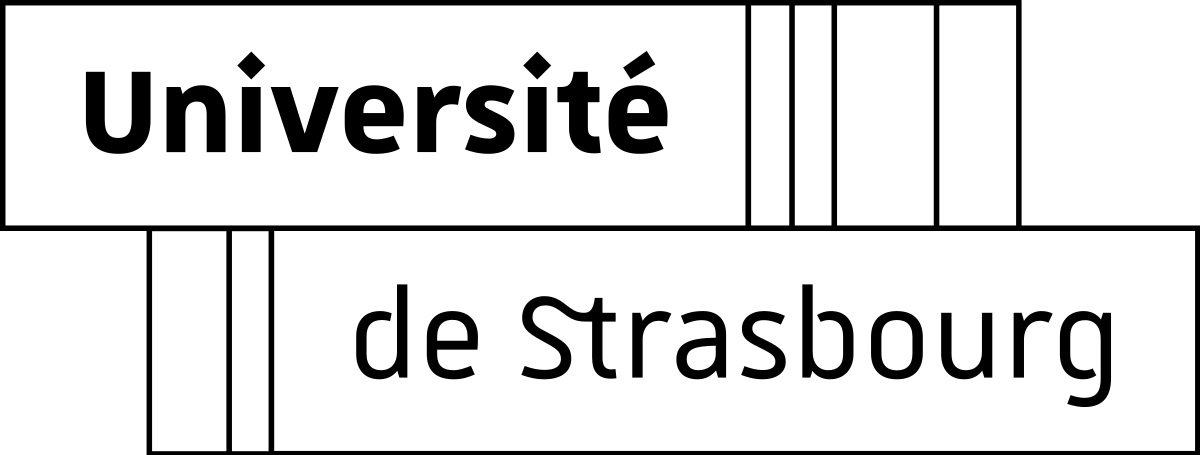
\includegraphics[width=0.4\textwidth]{SCHEMA/unistra.png}\par\vspace{1cm}
	{\scshape\LARGE University of Strasbourg\par}
	\vspace{1.5cm}
	{\huge\bfseries Monte Carlo Radiative Transfer in Astrophysics\\
	\par}
	\vspace{1cm}
            
\includegraphics[width=0.45\textwidth]{SCHEMA/grover_2.jpeg} \\
            %\includegraphics[width=0.35\textwidth]{SCHEMA/242484832_991562868306671_1226694600988047991_n.jpg} \\

	%{\Large\itshape Groupe 11\par}
	\vspace{2cm}
	%{\Large\itshape February 8, 2022 and February 22, 2022\par}
	\vfill
	Composed by\par
	\textsc{GALOIS Pierre, GUICHARD Pierre, HARMANT Guillaume, \\
	FOK Yulia, BOROWSKI Davy, FENOY Quentin}

	\vfill

	{\large M1 S2 - 2021-2022 \par}
\end{titlepage}

\tableofcontents
\listoffigures
\newpage 


%\begin{center}
%\section*{Abstract}
%\end{center}
%\newpage
\begin{multicols}{2}

\section*{1.1 Introduction}
\quad When an astrophysical source emits a photon, before being received by the observer, it can be affected by the different elements present in the interstellar medium. Especially, it can be diffused or absorbed and a new photon can be created by emission. So, to fully understand the radiation emitted by this source, we also need to understand the behaviour and the nature of the interstellar medium over the line of sight. The optical depth, which describes the transmitted flux through a materials, is here the central quantity. This quantity allows us to characterize how easily the light can go through a given medium at a given wavelength.

However, characterizing all the diffusion over the path of the photon can be very hard. Indeed, to do that we need to detect and understand the scattering physics of all the different structures and mediums, the photon will go through along its path. Detecting it is an observational problem, but to understand their scattering physics, using numerical simulation can help us to get some information about the behaviour of the photon in a given medium. 


Here, our main goal is to create a numerical simulation of the scattering of photons inside a given medium based on a Monte-Carlo algorithm and to create a virtual telescope to detect what we see from the outside of the medium. This simulation will be created in python, we will test several conditions over the medium and see what is the impact over the path of a photon.

\section*{1.2 Theoretical aspect of radiative transfer. }





\quad Let's consider a source at a distance $d$ of the observer. We consider here a semi-classical model where photons are moving in straight line. We suppose there exists a medium of density $n$ along the line of sight between the sources and the observer. Interactions of this photon with a particle of this medium are probabilistic processes described by a cross section $\sigma$. The ratio of the transmitted flux over the total flux is called the optical depths and it's linked to the cross section and the density over the line of site by: 

\begin{align}
    \tau = \int _0 ^L \sigma(x)\cdot n(x)\dd x
\end{align}
Where $n$ is the particle density in x with a source in $0$ and the observer at a distance $L$ from it.

In a radial problem (where all quantities depend only of their radius from the origin), the behaviour of the intensity of a light beam at frequency $\nu$ is described by the radiative transfert equation: 

\begin{align}
\frac{\dd I_{\nu}}{\dd x}=j_{\nu}-\alpha _{\nu} ^{abs} \cdot I_{\nu} -\alpha _{\nu} ^{scat}\cdot (I_{\nu}-J_{\nu})
\end{align}
with: 
\begin{itemize}
    \item $\alpha _{\nu} ^{abs}=n \cdot \sigma_{\nu} ^{abs} =(l_{\nu} ^{abs})^{-1}$ where $\sigma _ {\nu} ^{abs}$ is the cross section of absorption of a photon of frequency $\nu$ and $l_{\nu} ^{abs}$ the mean free path of a photon before absorption. 
    
    \item $\alpha _{\nu} ^{scat}=n \cdot \sigma_{\nu} ^{scat} =(l_{\nu} ^{scat})^{-1}$ where $\sigma _ {\nu} ^{scat}$ is the cross section of scattering of a photon of frequency $\nu$ and $l_{\nu} ^{abs}$ the mean free path of a photon before scattering.
   \item $J_{\nu}$ the angular average of the intensity. In a isotropic case,  $J_{\nu}=I_{\nu}$. 
   \item $j_{\nu}$ the emission coefficient of the medium.  
\end{itemize}

This in-homogeneous first order differential equation describe the behaviour of the intensity of a beam of light inside a given medium. It can be easily solved with some assumption we will describe later. 

Several processes can occurs inside the interstellar medium. First, we can have scattering of a photon without lose of energy (Thomson or Rayleigh scattering). Scattering send the photon in random direction without changing $\nu$. It's occured for low energy photons. If our photons is high energy (x-ray or gamma-ray photon), we speak about Compton scattering, where the scattering follow a lose of energy of the photon. We can also have absorption and emission of photons by the medium following quantum mechanics. 

In the interstellar medium, all this process can occurs simultaneously. For instance, this is this kind of processes which define several type of nebulae and star forming region (emission nebula, absorption nebula or reflection nebula). Understand this phenomenon allow us to  probe the interstellar medium and understand what we see through a telescope. In addition, thanks to this, we can modelize radiative transfer inside a stars and get information on its structure. 




Finding the interaction points depends on the opacity in the medium. Along its trajectory, measured by $l$, a packet ($p$), continuously accumulates optical depth
\begin{align}
    \tau_p(l)=\int_0^l \dd l' \chi(l').
\end{align}
Here the specific functional form of the opacity depends on the physical interaction processes that are taken into consideration and can, in principle, be very complicated. When the accumulated optical depth surpasses a threshold value, $\tau$, the packet will undergo an interaction at the corresponding location $l$. This threshold value is determined for each packet individually and probabilistic. In particular, at the beginning of each packet trajectory segment, the packet is assigned a randomly sampled optical depth distance to the next interaction by
\begin{align}
    \tau = -\ln \xi.
\end{align}


\section*{1.4 How to compute the point of next scattering}

\textit{\quad When we finally reach $\tau_s >\tau$, we might have already overshot our target value. In order to avoid inaccurate behaviour of our simulation, it would be good to do an interpolation for the target point, using the data from that last interval. A linear interpolation would be good enough.} From \cite{Noebauer_2019} Eq. 32 :
\begin{align*}
    x=x_{i+1}-\frac{f_X(x_{i+1} )-\xi }{f_X(x_{i+1} )-f_X(x_i)}(x_{i+1}-x_i)
\end{align*}

\section*{1.5 Simulating a telescope}

\quad In order to simulate a telescope, we need the list of all the photons escaping the outer shell of the spherical scattering medium. 
For each photon we have to know its position $[x,y,z]$, as well as its direction $[vx, vy, vz]$.
As we want to increase the efficiency of our telescope, we do as if we rotated it around the scattering object, pointing towards the center. 

In order to simulate this, we suppose that the object has a rotational symmetry around the $z$ axis. Then, the vertical position of the photon on the image is given by its $z$ coordinate. To compute the horizontal coordinate we will need the following angles: 
\begin{enumerate}
    \item $\tan(\phi)=\frac{y}{x}$
    \item $\tan(\theta)=\frac{z}{r}$ where $r=\sqrt{x^2+y^2+z^2}$
    \item $\tan(\beta)=\frac{vy}{vx}$
\end{enumerate}

Then the horizontal position on the image is given by: 
$$x_{image}=r\sin(\beta-\phi)\cos(\theta)$$

Once we have these coordinates, we have to implement them in the program. 
To do so, we find the maximum value of $z$ and the maximum value of $x_{image}$ and we proceed as following: Our image is composed of N pixels in height and M pixels in length. We choose the highest position of the pixel for $z_{max}$ and the highest pixel in the horizontal ones for $x_{max}$



Idée pour la physique: 
\begin{enumerate}
    \item Considérer un milieu avec plusieurs especes chimiques différentes (donc une crosse section differentes).
    
    \item Se placer dans un cas plus generale avec un milieu absorbant le long de la ligne de vue. 
    
    \item Introduire une notion de longueurs d'ondes et de cross section qui depends de la longueurs d'ondes.
    
    \item Absorption de certains photons. 
    
    
\end{enumerate}
 


\newpage
\section{Numerical method}
\subsection{Monte Carlo generation}
\subsection{Inverse transform sampling}
Also known as Smirnov transform, it is the method for generating random numbers from any probability distribution given its cumulative distribution function.


\begin{mdframed}[style = solstyle]
\begin{small}
   \begin{tcolorbox}[colframe=black!5!white]
\textbf{Definition :}  

\textit{Probability distribution} : it is the mathematical function that gives the probabilities of occurrence of different possible outcomes for an experiment.
        \end{tcolorbox}
\end{small}
	\end{mdframed}

\begin{mdframed}[style = solstyle]
\begin{small}
   \begin{tcolorbox}[colframe=black!5!white]
\textbf{Definition :}  

\textit{Cumulative distribution function} : the cumulative distribution function of a real-valued random variable $X$, evaluated at $x$, is the probability that $X$ will take a value less than or equal to $x$.

        \end{tcolorbox}
\end{small}
	\end{mdframed}

\section{Checks of the consistency}

\subsection{Inverse transform sampling verification}
We can see that Fig. \ref{fig:planck_histo} has a the correct behavior.
\begin{Figure}
 \centering
 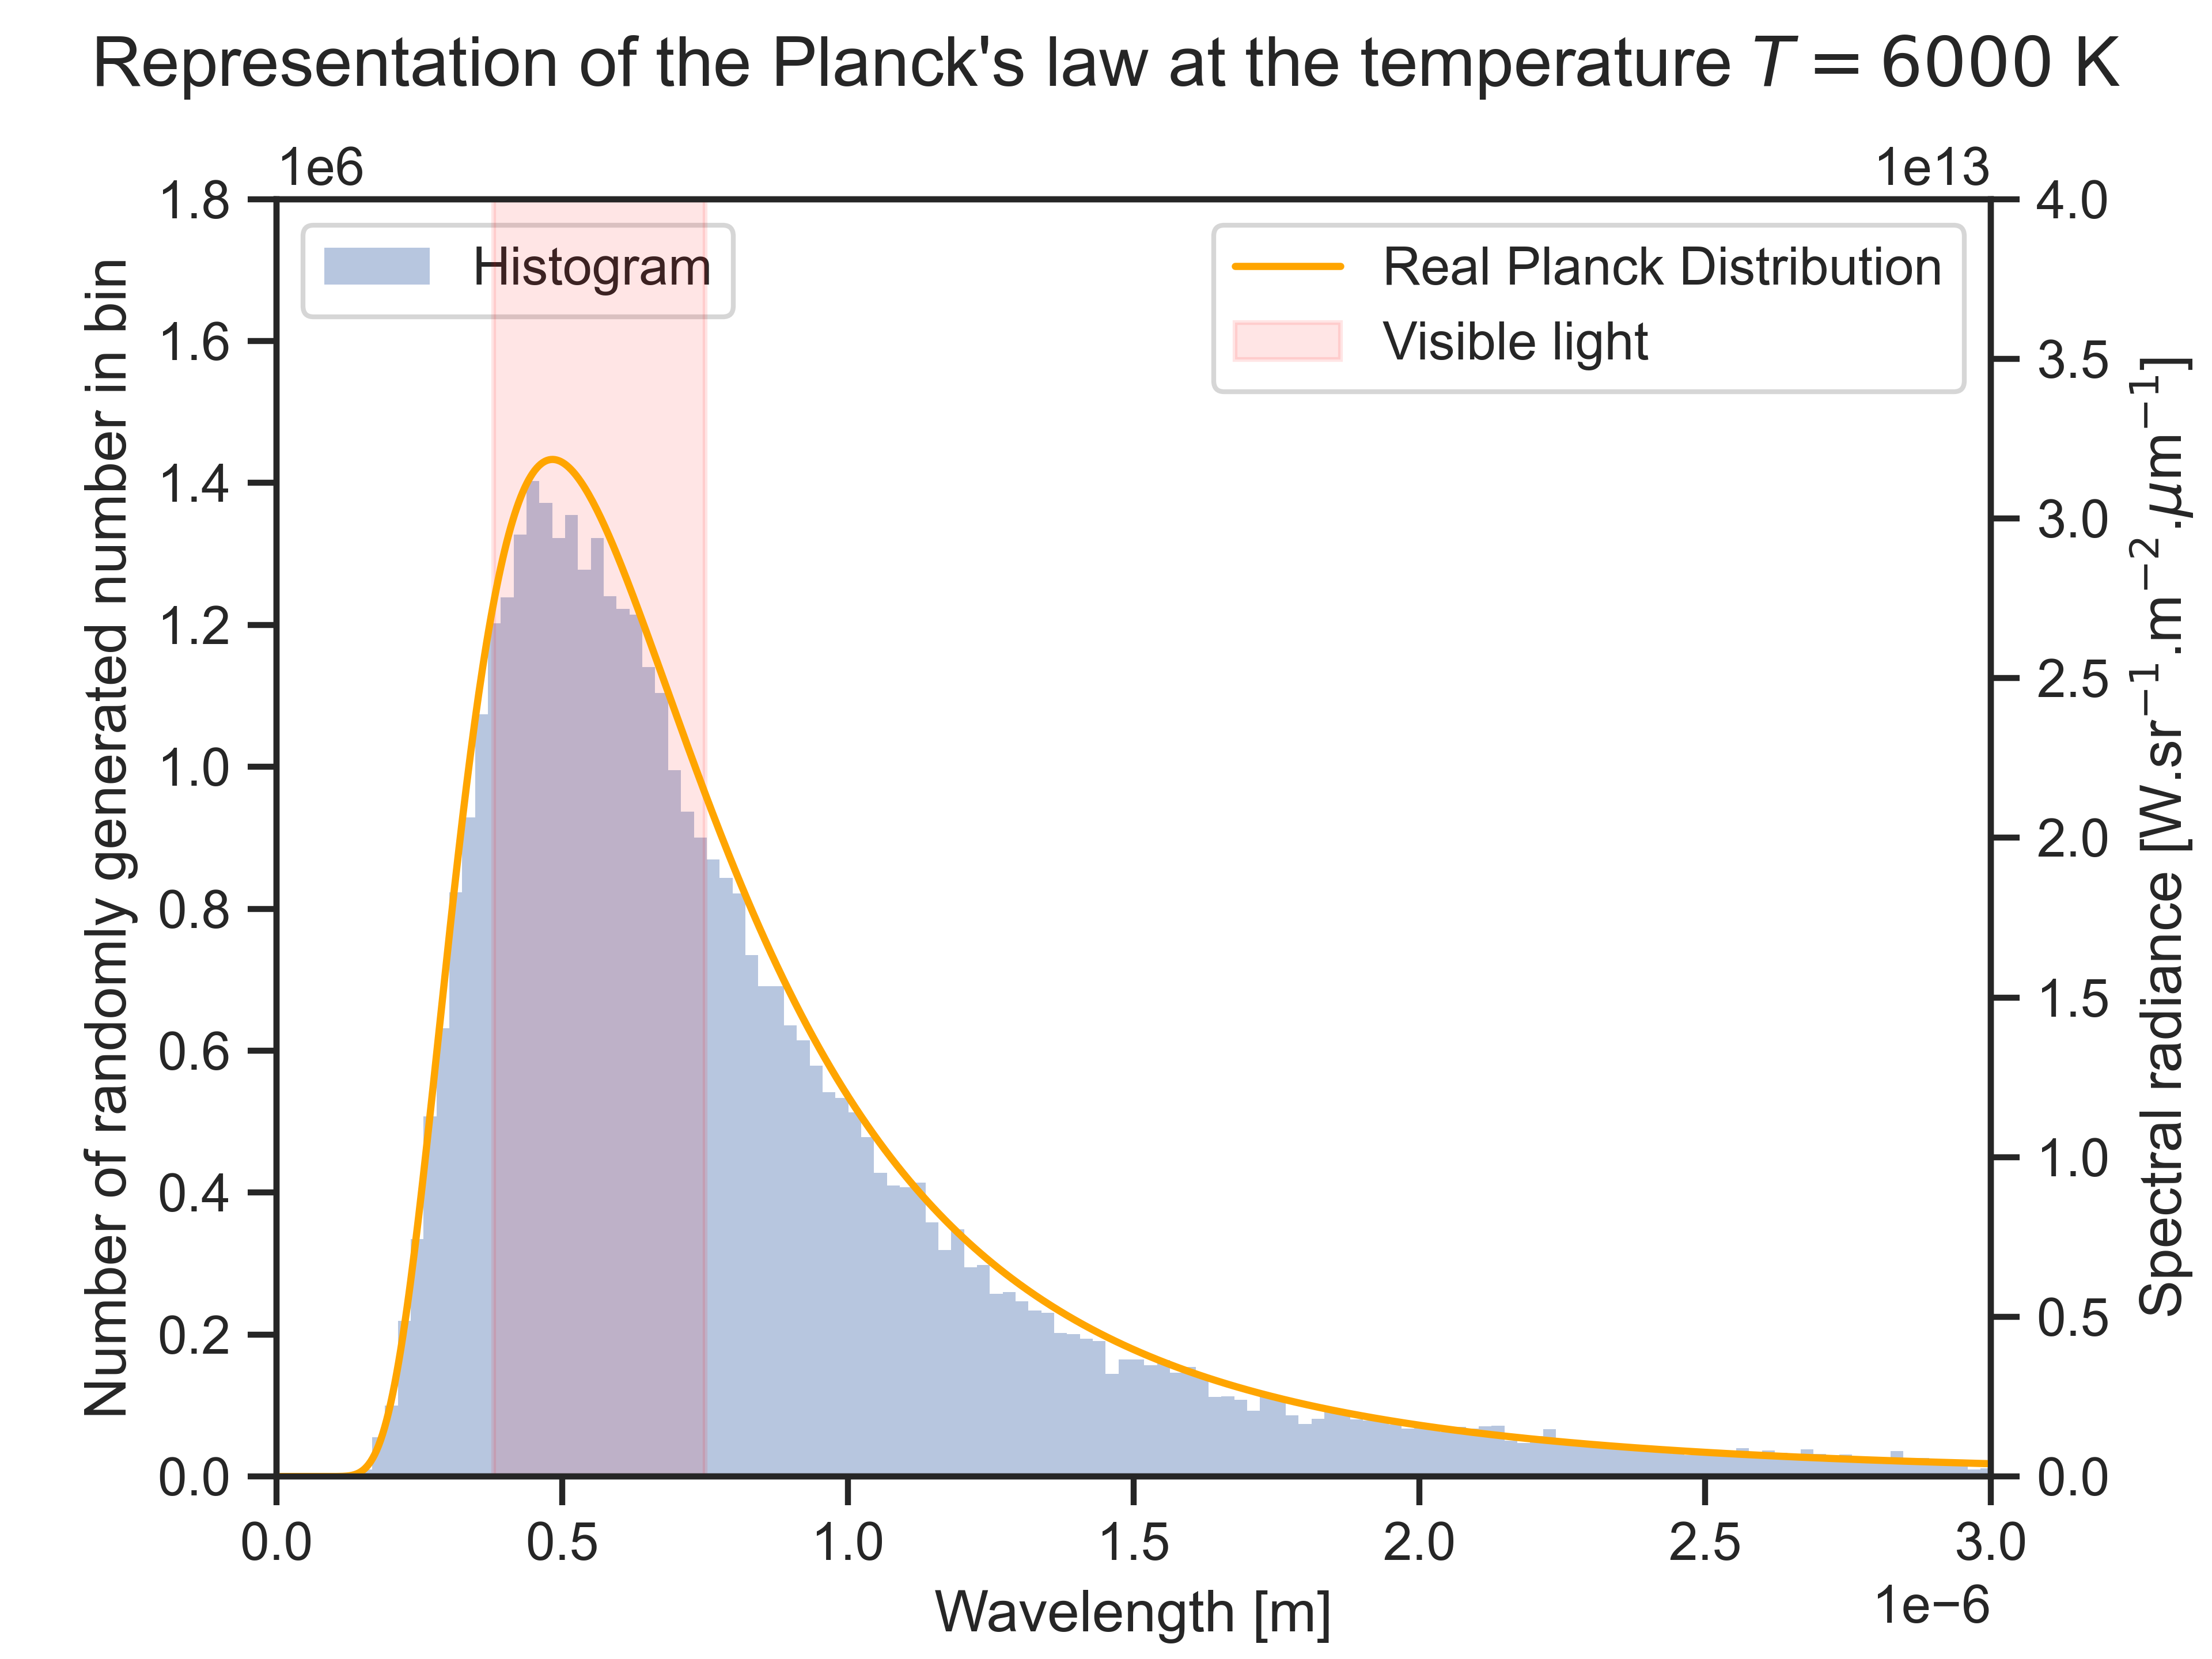
\includegraphics[width=1 \linewidth]{SCHEMA/planck.png}
 \captionof{figure}{Representation of the Planck's law at the given temperature $T=6000$ K. The blue histogram is generated randomly and the orange curve is the theoretical Planck's law.}
 \label{fig:planck_histo}
\end{Figure}

\end{multicols}











\clearpage

\bibliographystyle{unsrt}
\nocite{*}
\bibliography{bibliographie}

\clearpage
\begin{appendices}
\section{Appendices}

\end{appendices}
%%
%%
%%
%%
%%
%%
%%
%%
%%
%%
%%
\end{document}